\documentclass[12pt, a4paper]{article}

\usepackage[hmargin=2.5cm, vmargin=2cm]{geometry}
\usepackage{amsthm, amssymb, mathtools, yhmath, graphicx}
\usepackage{fontspec, type1cm, titlesec, titling, fancyhdr, tabularx}
\usepackage{caption}
\usepackage{color}
\usepackage{hhline}
\usepackage{unicode-math}

\usepackage[CheckSingle, CJKmath]{xeCJK}
\usepackage{CJKulem}
\usepackage{enumitem}
\usepackage[usenames, dvipsnames]{xcolor}
\usepackage{colortbl}
%\setCJKmainfont[BoldFont=cwTex Q Hei]{cwTex Q Ming}
%\setCJKsansfont[BoldFont=cwTex Q Hei]{cwTex Q Ming}
%\setCJKmonofont[BoldFont=cwTex Q Hei]{cwTex Q Ming}
\setCJKmainfont[BoldFont=cwTeX Q Hei]{cwTeX Q Ming}

\def\normalsize{\fontsize{12}{18}\selectfont}
\def\large{\fontsize{14}{21}\selectfont}
\def\Large{\fontsize{16}{24}\selectfont}
\def\LARGE{\fontsize{18}{27}\selectfont}
\def\Huge{\fontsize{20}{30}\selectfont}

\titleformat{\section}{\bf\Large}{\arabic{section}}{24pt}{}
\titleformat{\subsection}{\large}{\arabic{subsection}.}{12pt}{}
\titlespacing*{\subsection}{0pt}{0pt}{1.5ex}

\parindent=24pt

\DeclarePairedDelimiter{\abs}{\lvert}{\rvert}
\DeclarePairedDelimiter{\norm}{\lVert}{\rVert}
\DeclarePairedDelimiter{\inpd}{\langle}{\rangle}
\DeclarePairedDelimiter{\ceil}{\lceil}{\rceil}
\DeclarePairedDelimiter{\floor}{\lfloor}{\rfloor}

\newcommand{\unit}[1]{\:(\text{#1})}

\title{ \bf {\Huge 電子電路實驗二:KVL \& KCL}\\ 實驗預報}
\author{B02901178 江誠敏}
\date{2014/09/21}

\begin{document}

\maketitle

\section{預報問題}

\begin{enumerate}[itemsep=20pt, topsep=10pt]
	\item {\large 以 PSpice 或者其他各種電路模擬軟體,模擬圖 2.1 之電路,以求出各電阻的電流值與各電阻兩側之電位差的理論值。} \\[10pt]
\parbox{\linewidth}{\centering
		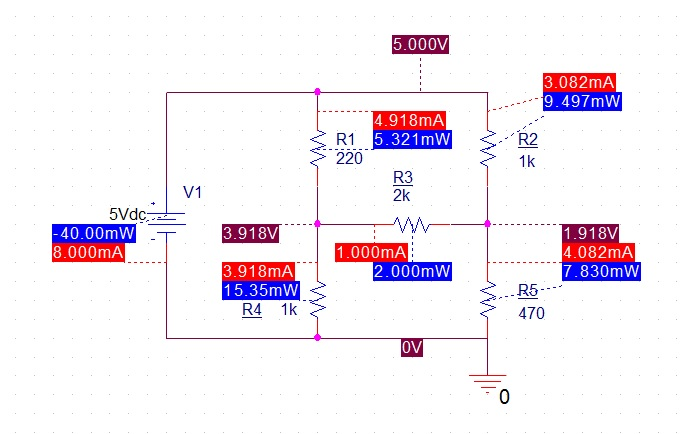
\includegraphics[width=10cm]{data/a1.jpg}
		\captionof{figure}{以PSpice模擬結果}
	} \\[10pt]
由Figure 1可以得到:
\begin{center}
\begin{tabular}{|p{4cm}|p{4cm}|p{4cm}|}
	\hline
	電阻 & 端電壓 & 電流 \\
	\hhline{|=|=|=|}
	R1 & $1.082 \unit{V}$ & $4.918 \unit{mA}$ \\
	\hline
	R2 & $3.082 \unit{V}$ & $3.082 \unit{mA}$ \\
	\hline
	R3 & $2.000 \unit{V}$ & $1.000 \unit{mA}$ \\
	\hline
	R4 & $3.918 \unit{V}$ & $3.918 \unit{mA}$ \\
	\hline
	R5 & $1.918 \unit{V}$ & $4.082 \unit{mA}$ \\
	\hline
\end{tabular}
\end{center}

	\item {\large 如何藉由電阻色碼來判斷電阻值?} \\[10pt]
		首先看電阻上的色碼有幾條,一般分為4碼與5碼。
		接著判斷色碼的頭尾方向:
		\begin{itemize}
			\item 4碼電阻:\ 由於4碼電阻的誤差通常較大,誤差的色碼通常為金、銀或無色,且這三種顏色不會在代表電阻的數值中出現,也就是說這三種顏色不會出現在第一環,因此可用其判斷方向。
			\item 5碼電阻:\ 通常代表誤差的色碼距離其它色碼較遠,可依此判斷。
		\end{itemize}
		最後查表,將色碼轉換成對應的數值:
		\begin{itemize}
			\item 4碼電阻:\ 假設對應的數值分別為$(a_1, a_2, a_3, a_4)$,代表此電阻的電阻值為\\$(10 a_1 + a_2 ) \times 10^{a_3}$,容許誤差為$a_4$。
			\item 5碼電阻:\ 假設對應的數值分別為$(a_1, a_2, a_3, a_4, a_5)$,代表此電阻的電阻值為$(100 a_1 + 10a_2 + a_3) \times 10^{a_4}$,容許誤差為$a_5$。
			\end{itemize}
			表格如下:\footnote{來源:實驗二的講義和wiki}
		\begin{center}
		\begin{tabular}{|p{3cm}|p{3cm}|p{3cm}|p{3cm}|}
\hline
黑 & $0$ & $10^{0}$ & \\
\hline
棕 & $1$ & $10^{1}$ & $\pm 1\%$ \\
\hline
紅 & $2$ & $10^{2}$ & $\pm 2\%$ \\
\hline
橙 & $3$ & $10^{3}$ & \\
\hline
黃 & $4$ & $10^{4}$ & \\
\hline
綠 & $5$ & $10^{5}$ & $\pm 0.5\%$ \\
\hline
藍 & $6$ & $10^{6}$ & $\pm 0.25\%$ \\
\hline
紫 & $7$ & $10^{7}$ & $\pm 0.1\%$ \\
\hline
灰 & $8$ &  & $\pm 0.05\%$ \\
\hline
白 & $9$ &  & \\
\hline
金 &  & $10^{-1}$ & $\pm 5\%$ \\
\hline
銀 &  & $10^{-2}$ & $\pm 10\%$ \\
\hline
無色 &  &  & $\pm 20\%$ \\
\hline
		\end{tabular}
		\end{center}

		\item {\large 請抽空到電子零件賣場(如台北光華商場附近就有很多電子零件賣場),看看市售的各種5\% 誤差固定電阻的電阻值(無須自行購買;強烈建議多看幾家)。記錄市售 5\% 誤差電阻的各種第一環與第二環的組合。(本題可於結報問題 6 一併回答。) } \\[10pt]
		將在結報問題6中一併回答。
\end{enumerate}

\end{document}

